\documentclass[8pt]{beamer}
\usetheme{Goettingen}
\usecolortheme{dove}
\setbeamercovered{transparent}
\setbeamerfont{frametitle}{size=\normalsize}
\setbeamertemplate{footline}[frame number]
\setbeamertemplate{itemize items}[circle]

\usepackage{mathrsfs} % equations
\usepackage{graphicx} % images
\usepackage[square,numbers]{natbib} % citations + references
\bibliographystyle{unsrtnat} % citations + references


\title{Drift Diffusion Model of Decision Making}
\author[]{Gabriel Riegner}
\date{March 2025}

\begin{document}

% slide %
\begin{frame}{Drift Diffusion Model of Decision Making}
\small
\begin{columns}
\column{0.5\textwidth}
\tableofcontents[hideallsubsections]
\column{0.5\textwidth}
\visible{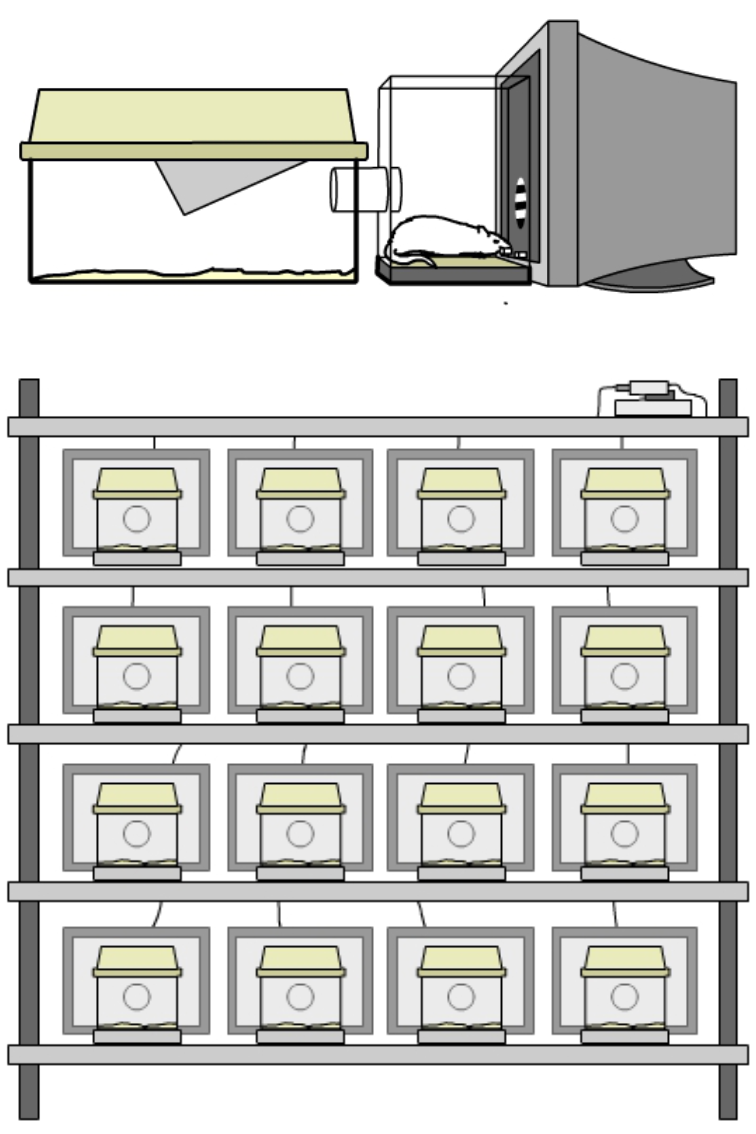
\includegraphics[width=0.8\textwidth]{docs/slides/figures/toc.png}}
\end{columns}
\vfill\centering
Gabriel Riegner (work with Pamela Reinagel, Armin Schwartzman)\\
UC San Diego, March 2025
\end{frame}

% section %
\section{Experimental Design}

% slide %
\begin{frame}{Experimental Design}
    \centering
    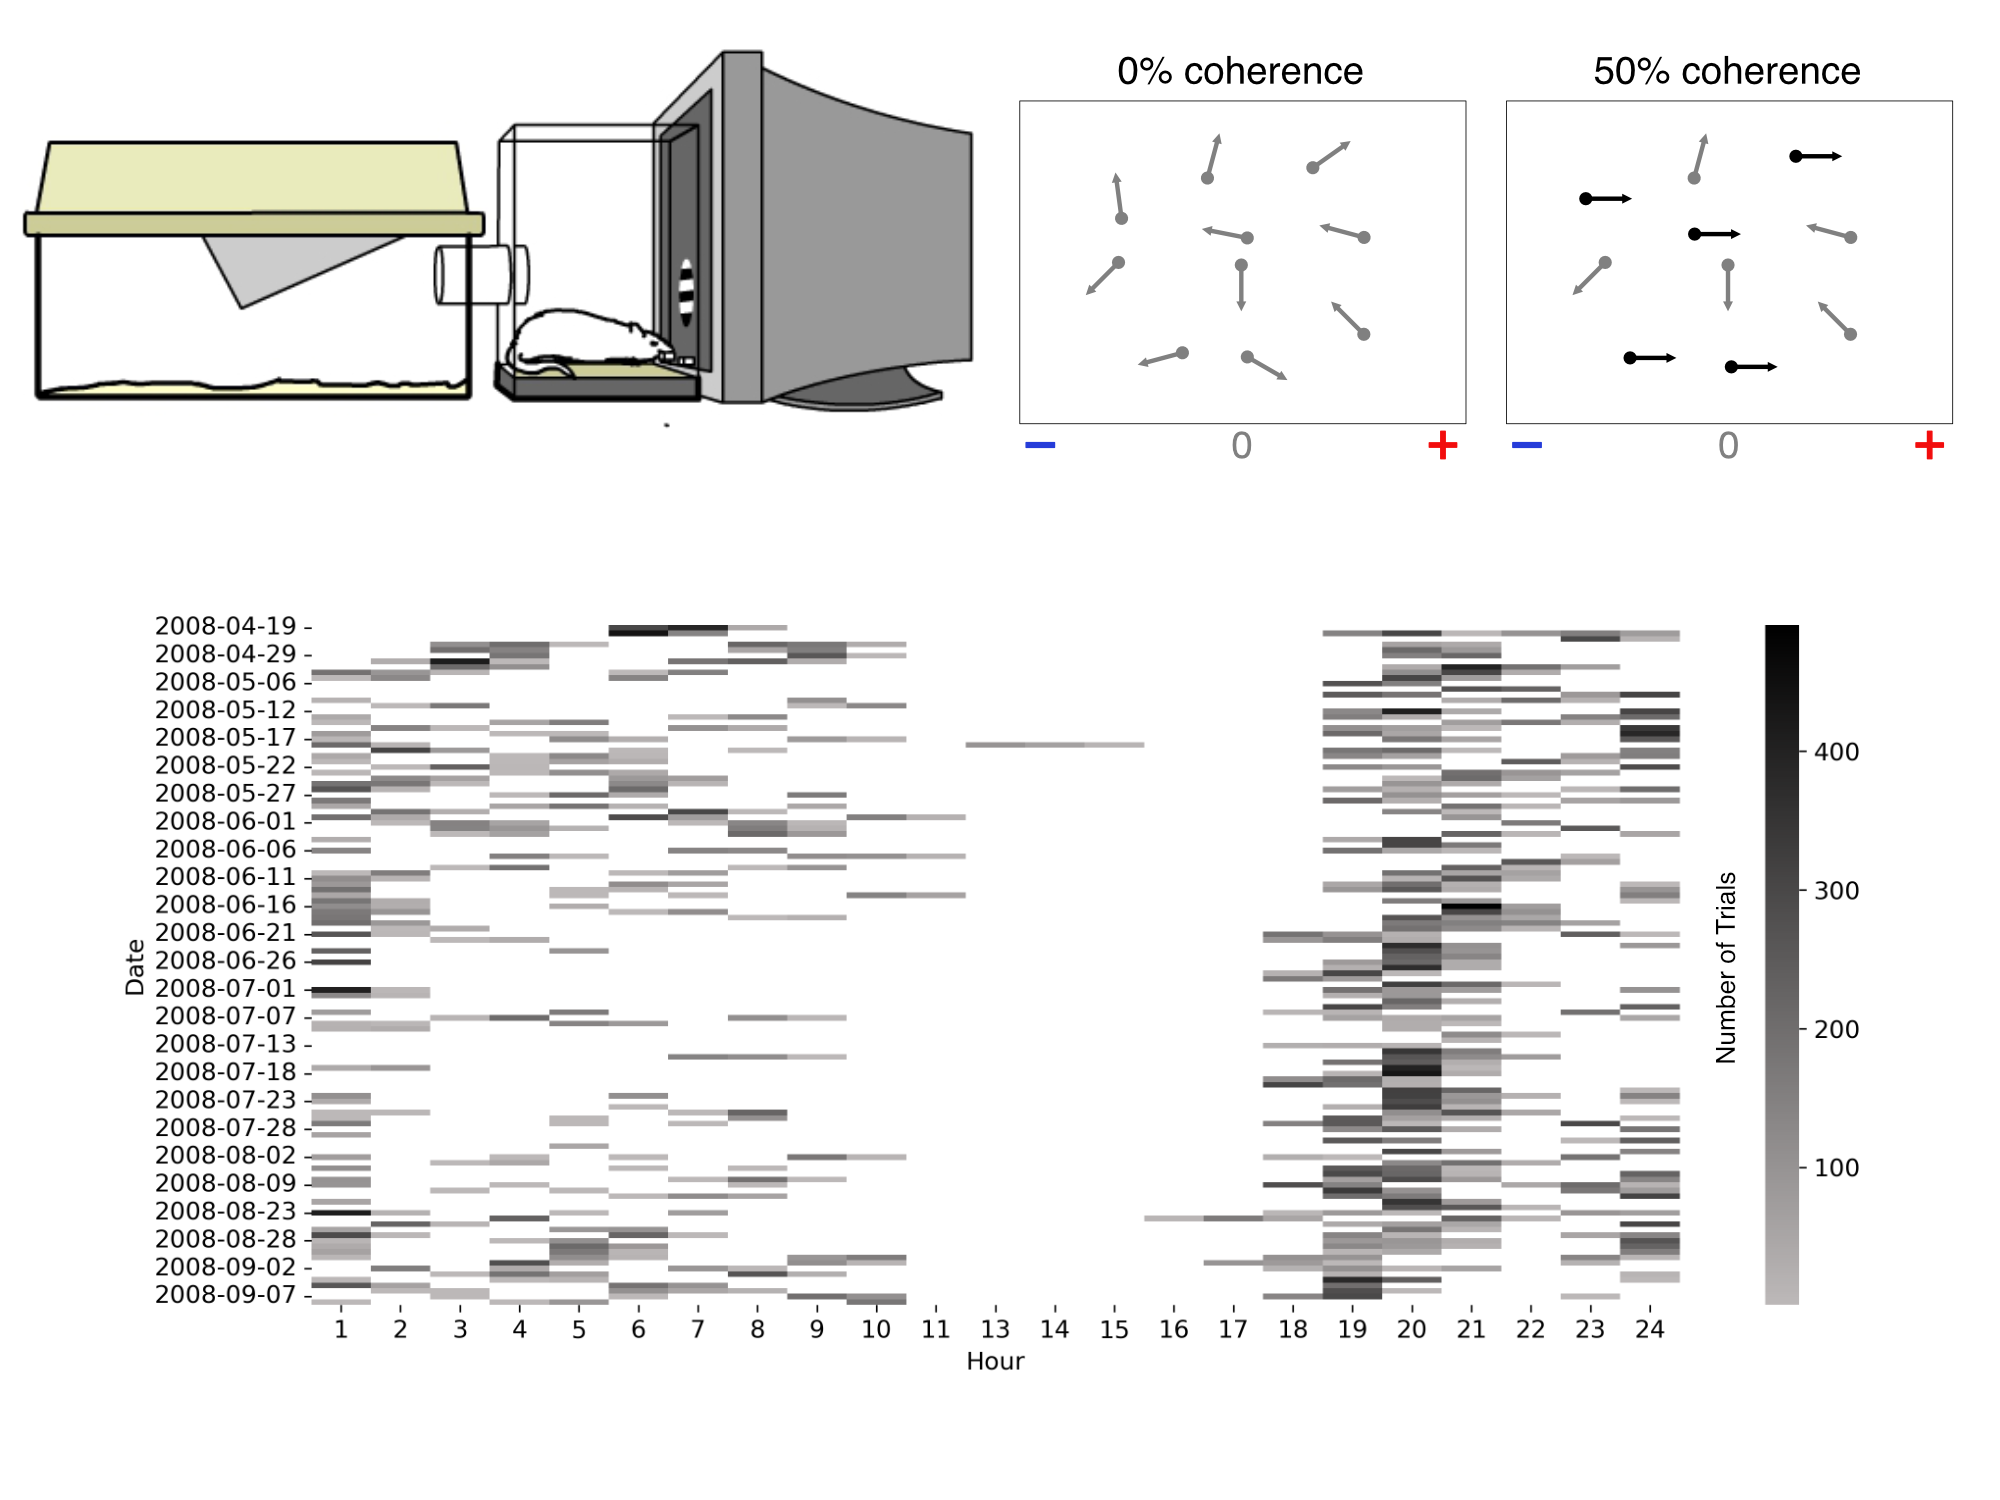
\includegraphics[width=1\textwidth]{docs/slides/figures/experimental-design.png}
    \small\href{https://www.ratrix.org/images/RatDotMotion.mp4}{[dot motion example]}
\end{frame}

% section %
\section{Drift Diffusion Model}

% slide %
\begin{frame}{Brain and Behavior}
    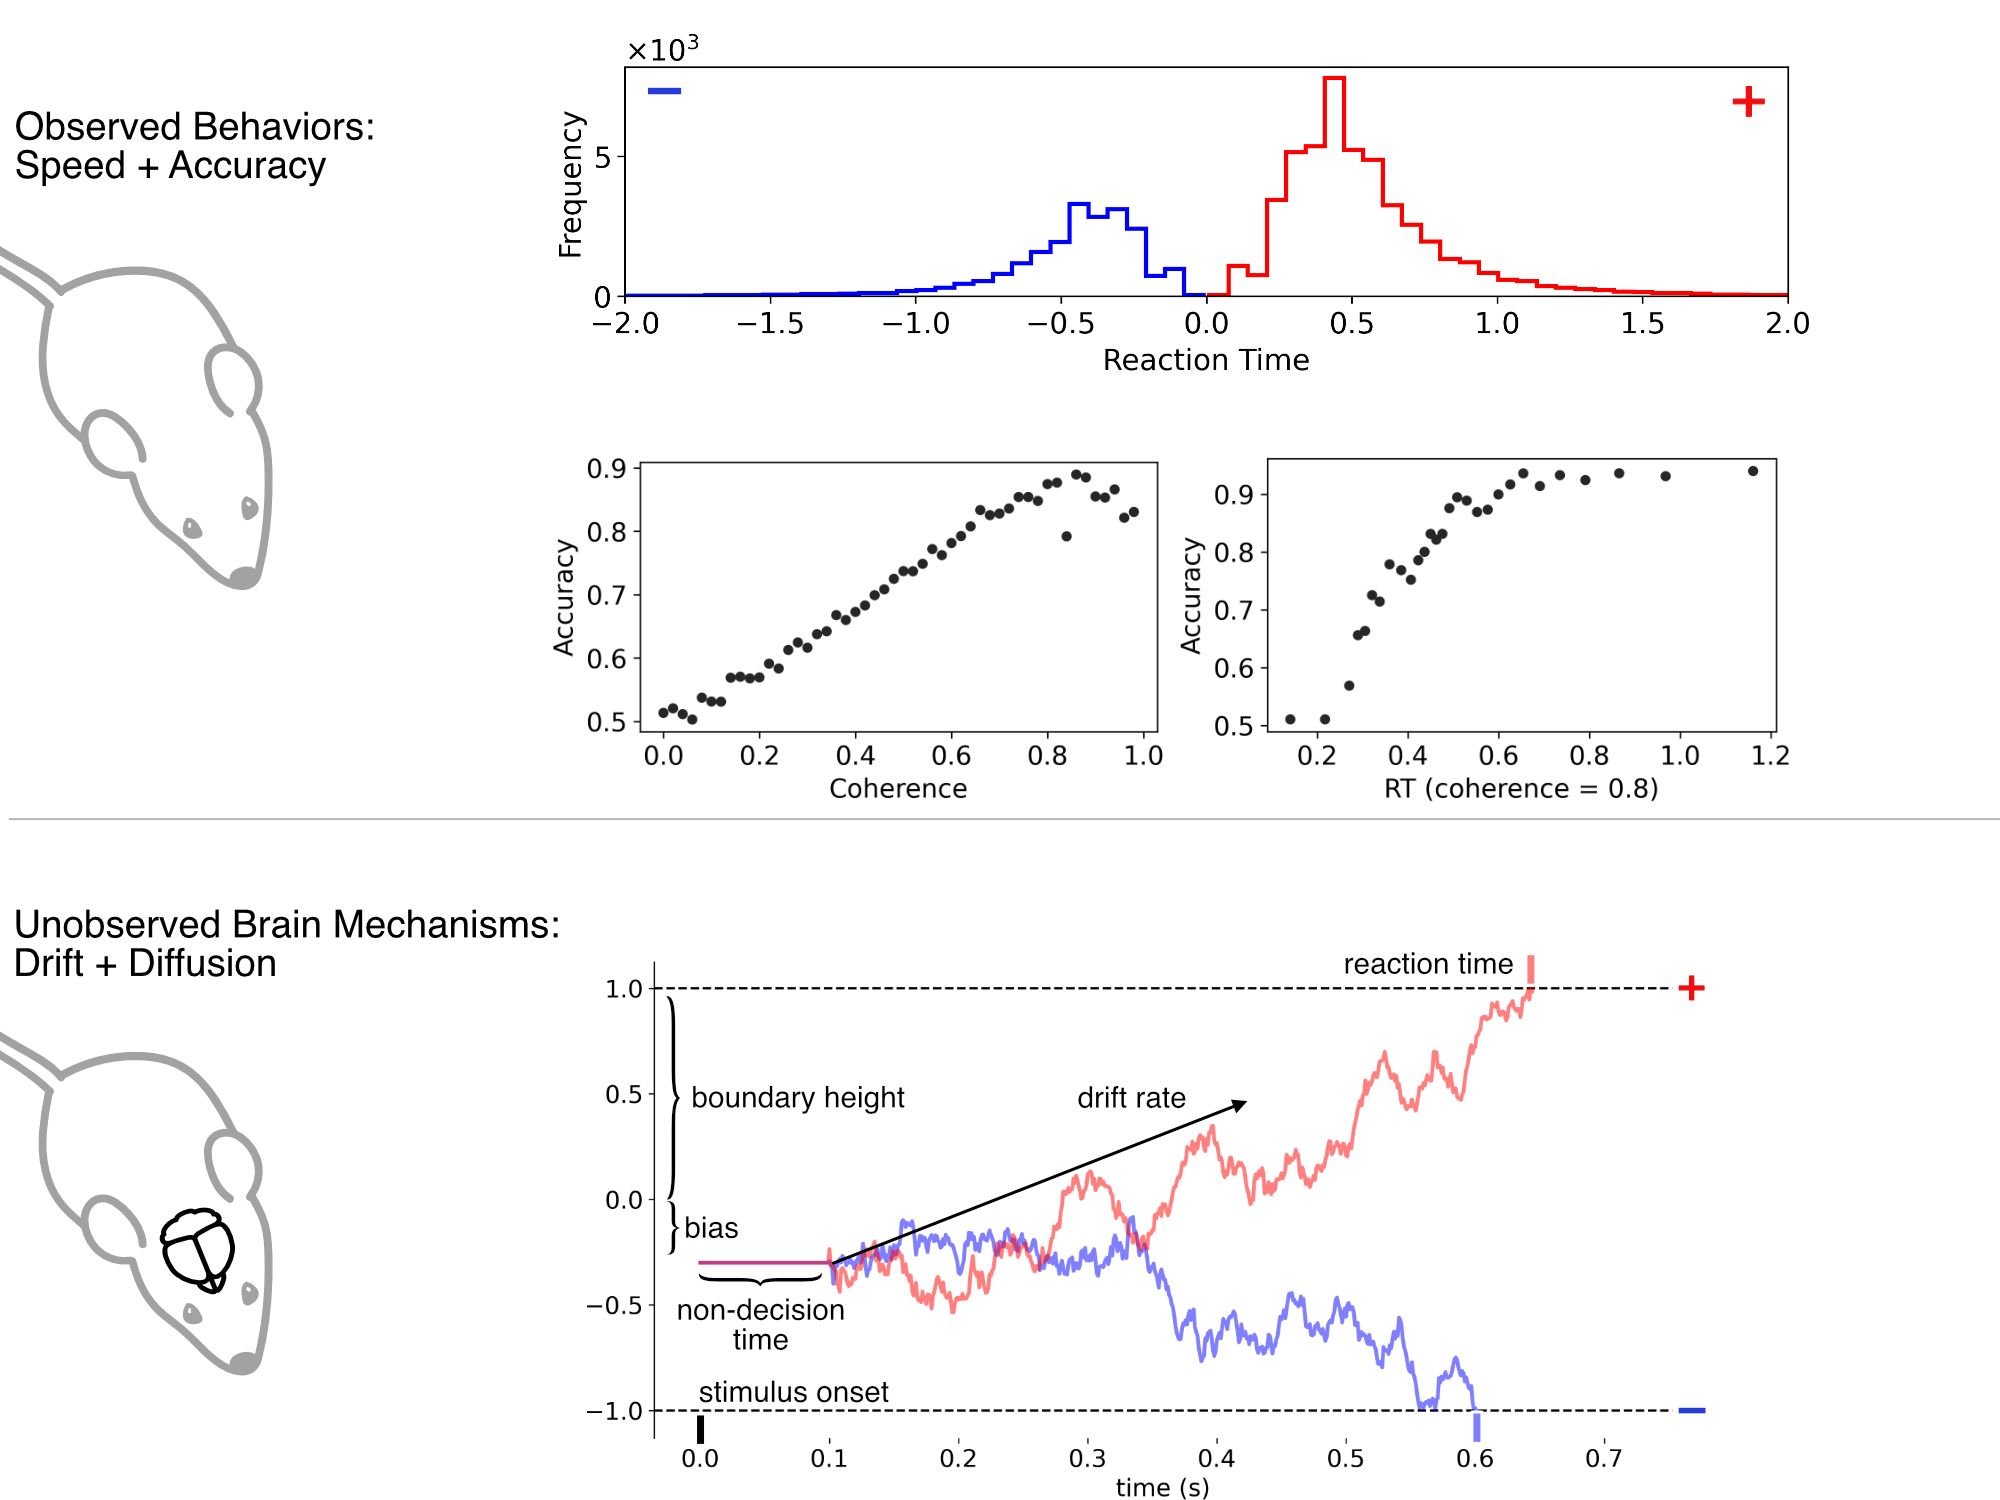
\includegraphics[width=1\textwidth]{docs/slides/figures/brain-behavior.png}
\end{frame}

% slide %
\begin{frame}{Drift Diffusion Model}
    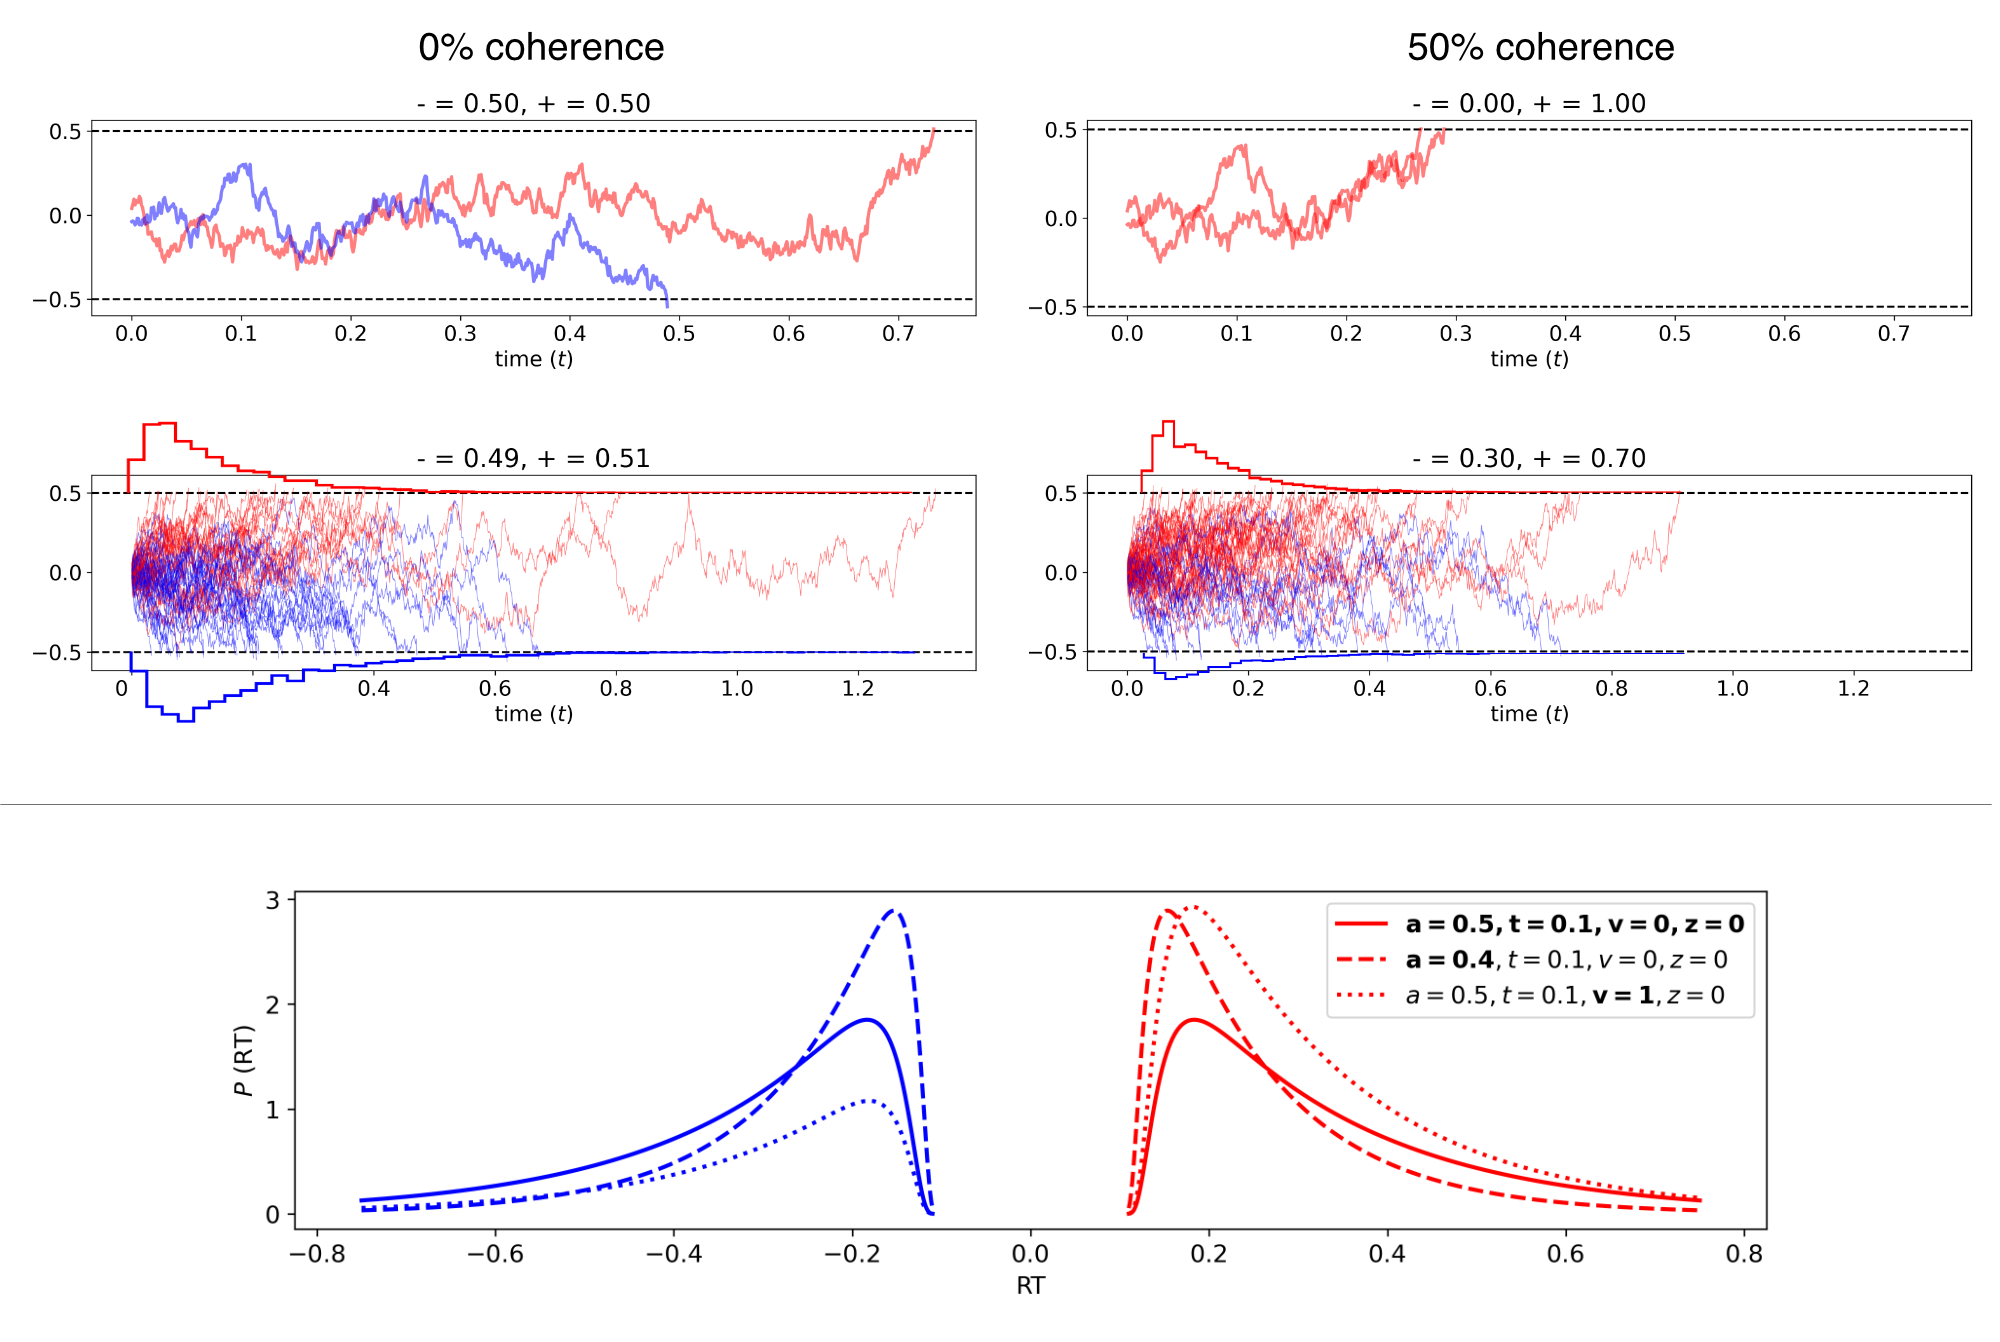
\includegraphics[width=1\textwidth]{docs/slides/figures/ddm-intuition.png}
\end{frame}

% slide %
\begin{frame}{Notation}
\textbf{Drift Diffusion Model}
\begin{align}
    Z_\tau = Z_{\tau-1} + e_\tau, \quad e_\tau \sim \mathcal{N}(v\Delta \tau, \sigma^2 \Delta \tau)
\end{align}
$v \in \mathbb{R}$ is the drift rate\\
$\Delta \tau \to 0$ is a continuous \textit{drift diffusion} process\\

\vspace{.25cm}
\textbf{RT + Response for} $\{Z_\tau: \tau=0, .., RT\}$
\begin{align}
    RT = \begin{cases}
        + \text{min}\{\tau>0: Z_\tau \ge +a\}\\
        - \text{min}\{\tau>0: Z_\tau \le -a\}
        \end{cases}
\end{align}
$a>0$ is the decision boundary\\
$|RT|> 0$ is the reaction time\\
$\text{sign}(RT) \in \{-1, +1\}$ is the response

\vspace{.25cm}
\textbf{RTs + Responses for} $\{Z_\tau: \tau=0, .., RT\}_t^T$
\begin{align}
    RT_t = \{RT_1, ..., RT_T\} \sim \mathcal{D}(a, v)
\end{align}

$t > 0$ is the trial time index\\
$\Delta t$ is nonconstant (unequally sampling)\\
$\mathcal{D}$ is probability distribution determined by parameters $a$ and $v$
\end{frame}

% section %
\section{Estimators}

% slide %
\begin{frame}{Definitions and Estimation}
\textbf{Probability Density Function}
\begin{align}
    f(RT \mid a, v) = \frac{\pi}{a^2}\exp\left(-\frac{va}{2}-\frac{v^2t}{2}\right) \times\sum_{k=1}^\infty k\exp\left(-\frac{k^2\pi^2 RT}{2a^2}\right)\sin(\frac{k\pi}{2})
\end{align}
from \citet{feller_introduction_1968, navarro_fast_2009}\\

\vspace{.25cm}
\textbf{Likelihood Function}
\begin{align}
    L_T(a, v \mid RT_t) = f(RT_t, ..., RT_T \mid a, v) = \prod_{t=1}^T f(RT_t \mid a, v)
\end{align}

\vspace{.25cm}
\textbf{Log-Likelihood Function}
\begin{align}
    \ell_T (a, v \mid RT_t) = \log L_T(a, v \mid RT_t) = \sum_{t=1}^T \log f(RT_t \mid a, v)
\end{align}

\vspace{.25cm}
\textbf{MLE} $\hat\theta$ of $\theta = (a, v)$
\begin{align}
    \hat\theta = \underset{\theta}{\text{argmin}} -\ell_T (\theta | RT_t)
\end{align}

\end{frame}


% slide %
\begin{frame}{Maximum Likelihood Estimator}
    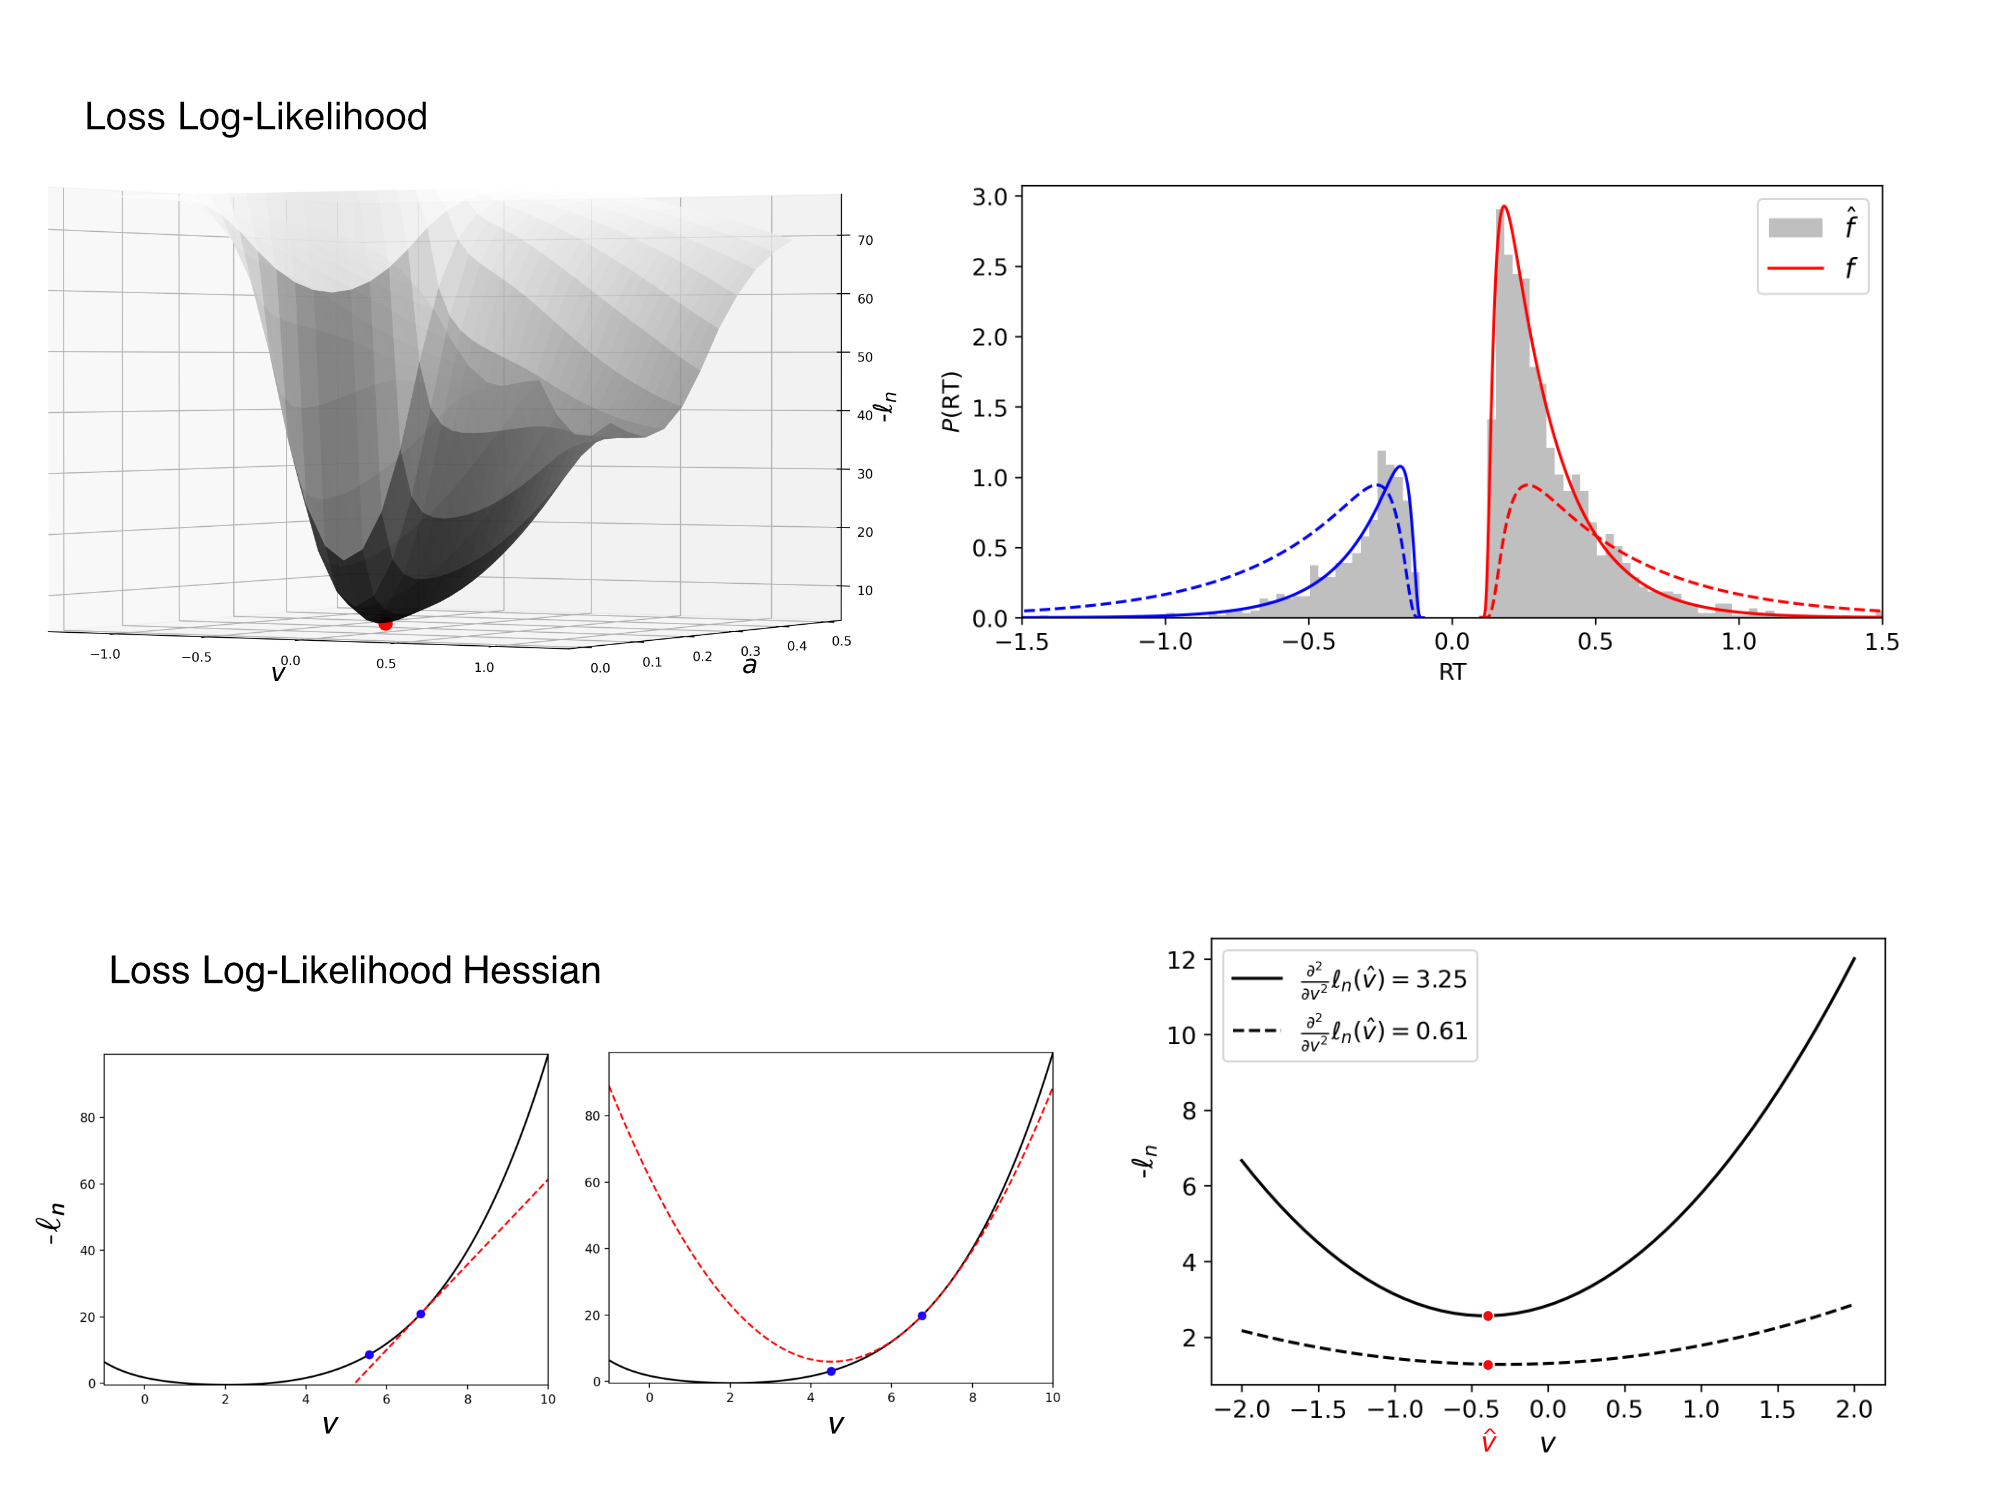
\includegraphics[width=1\textwidth]{docs/slides/figures/mle.png}
\end{frame}

% slide %
\begin{frame}{Asymptotic Covariance Estimators}

\begin{align}
    \widehat{\mathcal{H}}_\theta &= \frac{1}{T}\sum_{t=1}^T-\frac{\partial^2}{\partial\theta\partial\theta^{\prime}}\log f(RT_t\mid\hat{\theta})=-\frac{1}{T}\frac{\partial^2}{\partial\theta\partial\theta^{\prime}}\ell_T(\hat{\theta})\\
    \widehat{\mathscr{I}}_\theta &= \frac{1}{T}\sum_{t=1}^T\left(\frac{\partial}{\partial\theta}\log f(RT_t\mid\hat{\theta})\right)\left(\frac{\partial}{\partial\theta}\log f(RT_t\mid\hat{\theta})\right)^{\prime} = \frac{1}{T} \sum_{t=1}^T \hat{S_t} \hat{S_t}^\prime
\end{align}

\textbf{(1) Sample Hessian}\\
\begin{align}
    \widehat V_1 = \widehat{\mathcal{H}}_\theta^{-1}
\end{align}
\textbf{(2) Outer Product}\\
\begin{align}
    \widehat V_2 = \widehat{\mathscr{I}}_\theta^{-1}
\end{align}
\textbf{(3) Misspecification Robust} $\mathscr{I}_\theta \ne \mathcal{H}_\theta$\\
\begin{align}
    \widehat V_3 = \widehat{\mathcal{H}}_\theta^{-1} \widehat{\mathscr{I}}_\theta \widehat{\mathcal{H}}_\theta^{-1}
\end{align}
\textbf{(4) Autocorrelation Robust}\\
\begin{align}
    \widehat V_4 = \widehat{\mathcal{H}}_\theta^{-1} \left(\frac{1}{T} \sum_{i,j=1}^T w_{|i-j|} \hat{S_i} \hat{S_j}^\prime\right) \widehat{\mathcal{H}}_\theta^{-1}
\end{align}

from \citet[Chapter~10]{hansen_probability_2022}

\end{frame}



% section %
\section{Simulations}

% slide %
\begin{frame}{Simulations}

\textbf{Setting}: $a=0.83, v=0.79$, $N=1000$ repeats, $T=900$ trials

    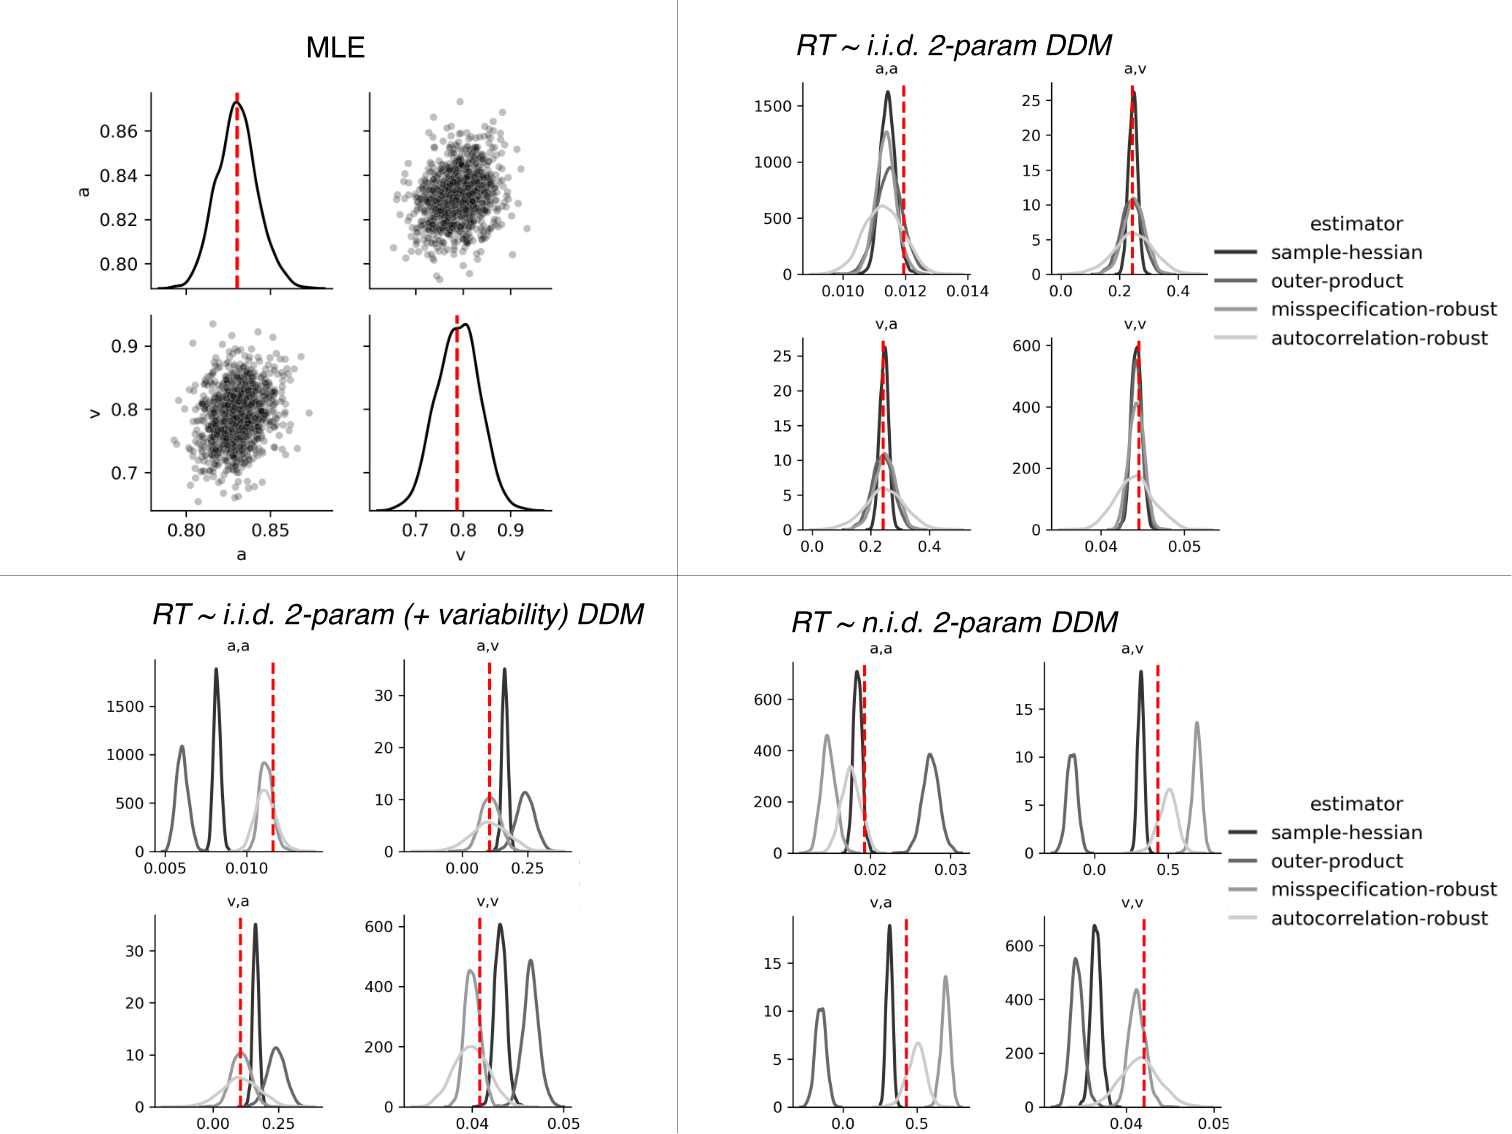
\includegraphics[width=1\textwidth]{docs/slides/figures/simulation-results.png}
\end{frame}


% section %
\section{Applications}

% slide %
\begin{frame}{Addressing Non-Stationarity}

\textbf{Dataset}: $N=1$ rat, $T=120k$ trials over $128$ days\\
\vspace{0.5cm}

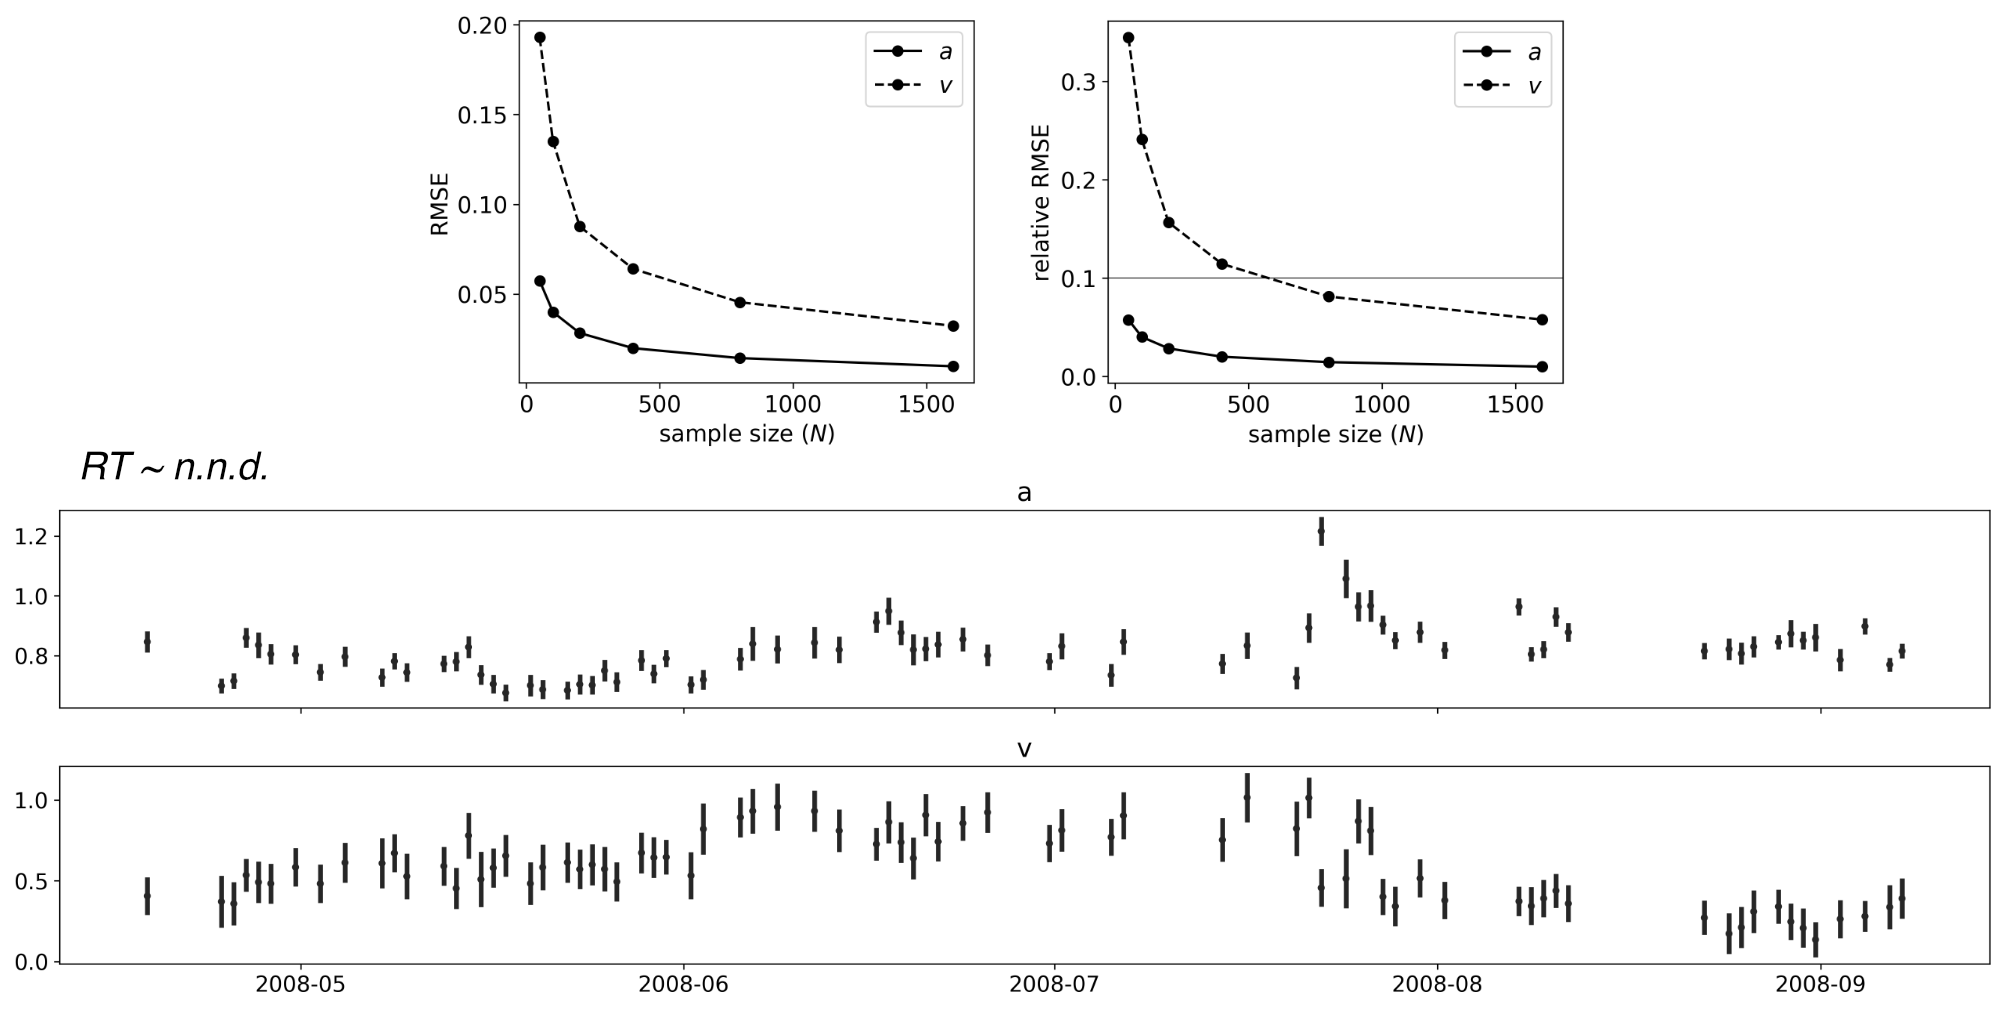
\includegraphics[width=1\textwidth]{docs/slides/figures/nonstationarity.png}

\citet{shevinsky_interaction_2019, nguyen_different_2022}
\end{frame}


% section %
\section{Conclusions}

% slide %
\begin{frame}{Conclusions and Future Directions}
    \begin{itemize}
        \item Drift diffusion model describes how brains process noisy information during two-choice decision tasks \vspace{0.25cm}

        \item MLE provides consistent point and interval estimators for model parameters and their standard errors from speed/accuracy behavioral data \vspace{0.25cm}

        \item Generalized estimation framework robust to model misspecification and autocorrelation in reaction times \vspace{0.25cm}

        \item Non-stationarity over time addressed by time-varying parameter estimation of freely behaving rats \vspace{0.25cm}

        \item Future work: Extending models to incorporate covariates explaining parameter changes over time
    \end{itemize}
\end{frame}

% slide %
\begin{frame}{References}
    \small
    \bibliography{docs/slides/zotero}
\end{frame}

\end{document}
